\documentclass[10pt]{PhDthesisPSnPDF}%
\usepackage{thesis_body}
\usepackage{pdfpages}

\usepackage{amsmath}%
\usepackage{amstext}%
\usepackage{amsfonts}%
\usepackage{amssymb}%
\usepackage{graphicx}
%\usepackage[latin1]{inputenc} 
\usepackage[T1]{fontenc}
\usepackage{authblk}
%\usepackage[bottom]{footmisc}
%\usepackage[top=3cm,left=2cm,right=2cm,bottom=2.5cm]{geometry} 
\usepackage[parfill]{parskip}
%\usepackage{titlesec}

%------------------------------------------------------------------
\hfuzz5pt % Don't bother to report overfull boxes < 5pt
\newtheorem{theorem}{Theorem}
\newtheorem{corollary}[theorem]{Corollary}
\newtheorem{definition}[theorem]{Definition}
\newtheorem{example}[theorem]{Example}
\newtheorem{exercise}[theorem]{Exercise}
\newtheorem{lemma}[theorem]{Lemma}
\newtheorem{proposition}[theorem]{Proposition}
\pagestyle{plain}
%%% --------------------------------------------------------------
\DeclareGraphicsExtensions{.jpg,.pdf,.mps,.png}

%\setcounter{tocdepth}{6}
%\setcounter{secnumdepth}{6}
%\setcounter{chapter}{1}

\title{\Huge{An introduction to \\ applied data science} \\ 
\rule{100mm}{5pt} \\
\Large{A 5-day workshop towards practical \\ big-data applications and analytics}}
%  with practical experience extracting value from big data
\author{\Large{Eduardo Barbaro}}
\author{\Large{Coen Jonker}}
\affil{\normalsize Data Scientistists at Mobiquity Inc}
\date{\today}

% ----------------------------------------------------------------------
% turn of those nasty overfull and underfull hboxes
\hbadness=10000
\hfuzz=50pt


%%%%%%%%%%%%%%%%%%%%%%%%%%%%%%%%%%%%%%%%%%%%%%%%%
% Start-up
%%%%%%%%%%%%%%%%%%%%%%%%%%%%%%%%%%%%%%%%%%%%%%%%%
\begin{document}

\renewcommand\baselinestretch{1}
\baselineskip=14pt plus1pt

\pagenumbering{roman}    %  roman numbering for all preamble pages
\maketitle

% ----------------------------------------------------------------

\noindent{\textbf{About the workshop and this manual:}} \\

Welcome to ``An introduction to applied data science'' a 5-day original workshop thought and written by Eduardo Barbaro and Coen Jonker. At the end of this week you will be able to (i) understand the basics of data science, (ii) mathematically describe data, and (iii) munge\footnote{describes the constructive operation of tying together systems and interfaces that were not specifically designed to interoperate} it into an easy and communicable form. As the course develops, we will teach you how to access and look at data in innovative ways, as well as to extract value from big data. We aim a significant part of this training to help you to create/interpret a diverse set of numerical models, as well as to calculate descriptive analytics while fully understanding their meaning. We also focus on presentation, and how to show your results in beautiful smart charts and tables.

<<<<<<< HEAD
Although all the computations will be performed in Mobiquity's AWS cloud, we will guide you through all the necessary steps to install any software necessary for this course in your local machines. We use Mobiquity's AWS cloud to get the benefit of running our code in a fast, secure, and controlled environment.

This manual is divided in 11 independent short chapters. In Chapter \ref{DS} we set the stage with a short introduction to then answer together a bold question: ``But what is data science?''. In Chapter \ref{basics} we will spend some time to recap some basic mathematical concepts needed throughout the entire workshop. Chapters \ref{P1} and \ref{P2} are devoted to (important) practicalities, such as installing software/libraries and getting familiar with the AWS cloud environment. We also teach you some basic programming skills, so we are all on the same page. We move forward to our first data harvest, in Chapter \ref{harvesting}. We teach you how to manipulate data, as well as to properly describe and clean it. Chapter \ref{numerics} covers the basics of designing a smart numerical experiment. 

Chapters \ref{MLearn} to \ref{bigData} cover more advanced topics such as machine learning tools, databases (SQL and no-SQL) as well as a mapreduce implementation (Hadoop). In particular, in Chapter \ref{bigData} we show in detail how to load, transform, and extract value from real big data. Finally, in Chapter \ref{Commun} we come back to basics to show you rudiments of plotting and how to communicate your results. 
=======
This manual is divided in 11 independent short chapters. In Chapter \ref{DS} we set the stage with a short introduction to then answer together a bold question: ``But what is data science?''. In Chapter \ref{basics} we will spend some time to recap some basic mathematical concepts needed throughout the entire workshop. Chapters \ref{P1} and \ref{P2} are devoted to (important) practicalities, such as installing software/libraries and getting familiar with the AWS cloud environment. We also teach you some basic programming skills, so we are all on the same page. We move forward to our first data harvest, in Chapter \ref{harvesting}. We teach you how to manipulate data, as well as to properly describe and clean it. Chapter \ref{numerics} covers the basics of designing a smart numerical experiment. 

Chapters \ref{MLearn} to \ref{bigData} cover more advanced topics such as machine learning tools, databases (SQL and no-SQL) as well as a mapreduce implementation (Hadoop). In particular, in Chapter \ref{bigData} we show in detail how to load, transform, and extract value from real big data.

Finally, Chapter \ref{Commun} covers the basics of plotting and communicating results. Although all the computations will be performed in Mobiquity's AWS cloud, we will guide you through all the necessary steps to install any software necessary for this course in your local machines. We use Mobiquity's AWS cloud to get the benefit of running our code in a fast, secure, and controlled environment.
>>>>>>> 605bbafd91b995bfdee82fc6aeefbd83e35910e4

We wish you a pleasant learning!

\newpage
\thispagestyle{empty}
\mbox{}
\cleardoublepage

% Counting	
%\setcounter{page}{1}
\setcounter{tocdepth}{2}


%%%%%%%%%%%%%%%%%%%%%%%%%%%%%%%%%%%%%%%%%%%%%%%%%
% Table of contents
%%%%%%%%%%%%%%%%%%%%%%%%%%%%%%%%%%%%%%%%%%%%%%%%%

%{\baselineskip=.8\baselineskip % shortens the spacing between lines in the TOC

\setcounter{secnumdepth}{3} % organisational level that receives a numbers
\setcounter{tocdepth}{2}    % print table of contents for level 3
\tableofcontents            % print the table of contents


%%%%%%%%%%%%%%%%%%%%%%%%%%%%%%%%%%%%%%%%%%%%%%%%%
% List of Figures and Tables
%%%%%%%%%%%%%%%%%%%%%%%%%%%%%%%%%%%%%%%%%%%%%%%%%
	
%\addcontentsline{toc}{chapter}{List of Figures}
%\listoffigures 
%\cleardoublepage
%\addcontentsline{toc}{chapter}{List of Tables}
%\listoftables 
%\cleardoublepage

%%%%%%%%%%%%%%%%%%%%%%%%%%%%%%%%%%%%%%%%%%%%%%%%%
% Chapters 
%%%%%%%%%%%%%%%%%%%%%%%%%%%%%%%%%%%%%%%%%%%%%%%%%

\cleardoublepage
% Introduction
\newpage
\pagenumbering{arabic}	 %  arabic numbering for all preamble pages

<<<<<<< HEAD
\chapter{A historical view on data science}\label{DS} 

In this Chapter we briefly try to shed some light on the question ``what is data science?''. First of all, it is important to realize that data science is not a new concept. There are many complex definitions out there, but in our view, data science is simply the coupling of very well-established disciplines, such as mathematics and statistics, with a relatively young discipline, computer sciences. 

Have a look at Fig. \ref{fig:Analytics}. It shows the evolution of 5 fundamental disciplines related to data science (Mathematics, Statistics, visualization, technology, computer science). Note that this cartoon depicts events as old as the ``invention'' of modern calculus by Newton/Leibniz (in the 17$^{th}$ century) or foundation of probability theory by Cardano (in the 16$^{th}$ century). You can see that back in those times all the disciplines were really self-contained areas without much interconnection. As we enter the 20$^{th}$ century things start to get more interconnected. Statistics and Mathematics cannot be separated so clearly any more (e.g. stochastic models, survival models), and computer sciences and technology started to gain more terrain. 
\newpage
\begin{figure}[h]
	\begin{center}
			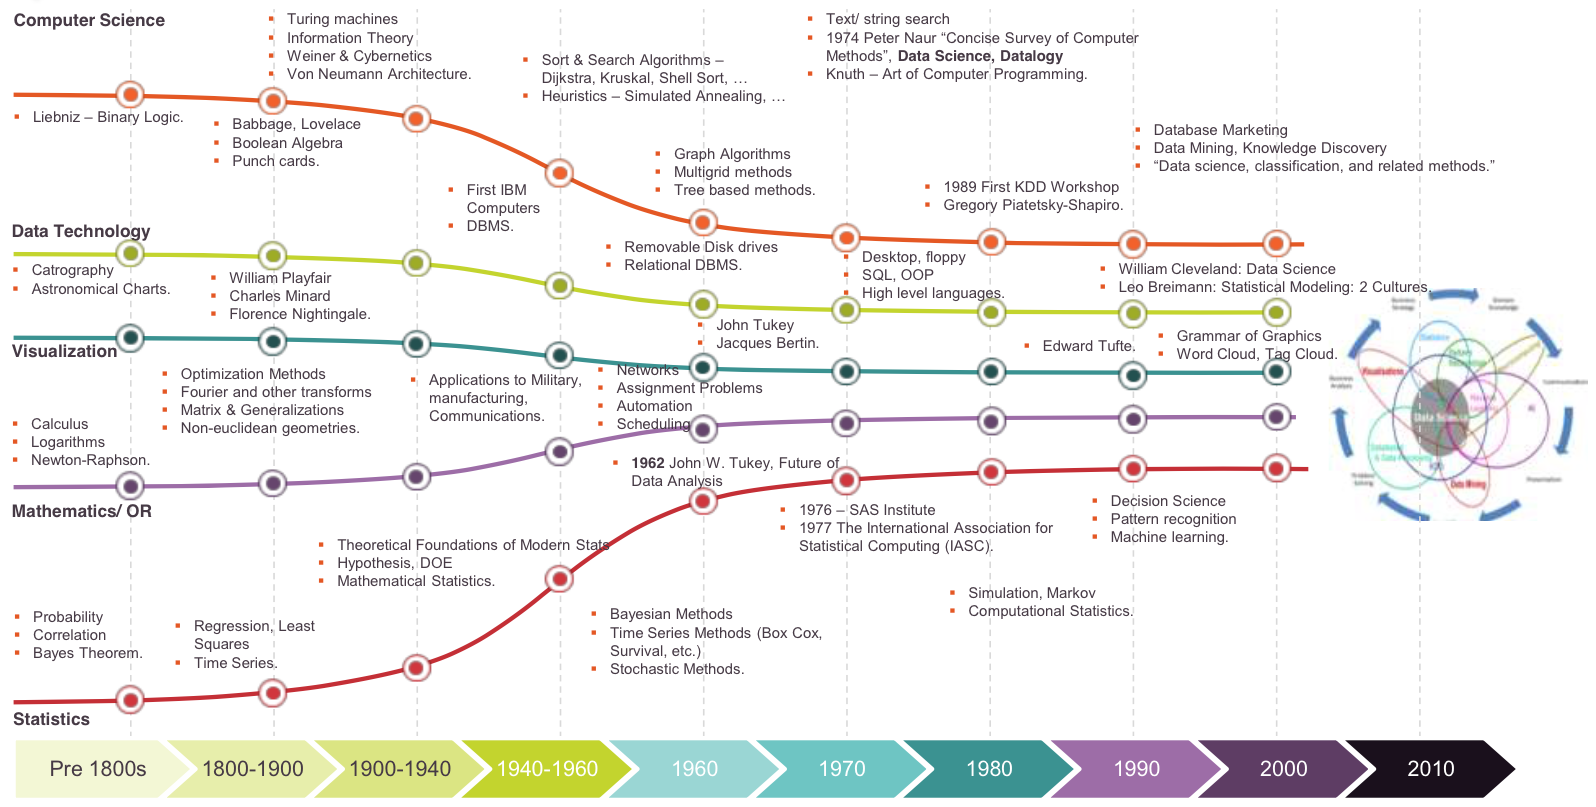
\includegraphics[scale=0.25]{HistoryCH1}
	\end{center}
	\caption{Most important events in the history of data science. \textit{Credit: Mamatha Upadhyaya}}
	\label{fig:Analytics}
\end{figure} 

As early as 1962, John Wilder Tukey, an American Mathematician, wrote in his ``The future of data'':
\begin{quotation}
\textit{For a long time I thought I was a statistician, interested in inferences from the particular to the general. But as I have watched mathematical statistics evolve, I have had cause to wonder and doubt. I have come to feel that my central interest is in data analysis. Data analysis, and the parts of statistics which adhere to it, must take on the characteristics of science rather than those of mathematics data analysis is intrinsically an empirical science.}
\end{quotation} 
 
That served as inspiration to Tukey who, in 1977, published his most well-known book ``Exploratory Data Analysis''. In that book, he argued that exploratory and confirmatory data analyses must proceed alongside. Also in the 1970's, Peter Naur, Danish computer science pioneer, published ``Concise Survey of Computer Methods''. In this book, the term data science was used for the first time. According to him, data science can be defined as:
\begin{quotation}
\textit{The science of dealing with data, once they have been established, while the relation of the data to what they represent is delegated to other fields and sciences.}
\end{quotation} 

In the beginning of the 21$^{st}$ century all the disciplines related to data science merged. In 2008, Jeff Hammerbacher (Facebook) and DJ Patil (LinkedIn) used the terminology ``Data scientist'' to define their work and teams. Since then, the use of this terminology has fully infiltrated the vernacular, and did not stop growing. 

Today, data science and computer sciences (through machine learning) have been put together as almost synonyms. There are new terminologies appearing every year, such as Deep Learning, Big Data, Data Mining. Today, we understand that data science and big data do not mean (just) ``lots of data''. Instead, it means the creation of a new paradigm in how we do analysis and combine the use of our traditional tools (Mathematics and Statistics) with the technology available nowadays.

 


=======
\chapter{But what is data science?}\label{DS} 
>>>>>>> 605bbafd91b995bfdee82fc6aeefbd83e35910e4
\chapter{Some basics and beyond}\label{basics}
\chapter{Practicalities: Software Installations and AWS cloud}\label{P1}
\chapter{Practicalities: Programming language and libraries}\label{P2}
\chapter{Harvesting data} \label{harvesting}
\section{Data Manipulation}\label{dataM} 
\section{Analytics 1: Describing your data}\label{Analy.1}
\section{Analytics 2: Cleaning your data}\label{Analy.2}
\chapter{Numerical Modeling}\label{numerics}
\section{Basics}\label{numBasics}
\section{Designing smart numerical experiments}\label{NumDesign}
\chapter{Machine learning tools}\label{MLearn}
\section{Supervised methods}
\section{unsupervised methods}
\chapter{Databases}\label{databases}
\section{SQL}
\section{NoSQL}
\subsection{MongoDB}
\chapter{Map Reduce}\label{mapR}
\section{Hadoop}
\chapter{Big Data}\label{bigData}
\chapter{Communicating Results}\label{Commun}
\section{Visuals}\label{Visuals}

%supervised learning (trees and forests, nearest neighbor, regression)
%optimization (gradient descent)
%unsupervised learning (clustering, )





%http://work.caltech.edu/telecourse


%\begin{equation}
%T=\frac{1}{2}\cdot \sum{(X_i - X_{i-1})\cdot(Y_i+Y_{i-1})}
%\label{eq:T}
%\end{equation}
%
%\
%   
%
%\begin{figure}[h]
%
%	\begin{center}
%		$\begin{array}{c@{\hspace{1in}}c}
%%			\includegraphics[scale=0.25]{Simpsons} &
%%			\includegraphics[scale=0.45]{Simpson} \\ [0.4cm]
%			\mbox{\bf (Homer Simpson)} & \mbox{\bf (Metodo de Simpson)}
%		\end{array}$
%	\end{center}
%	\caption{Metodo de Simpson}
%	\label{fig:Simpson}
%\end{figure}
%
%\pagebreak
%
%
%\begin{eqnarray}
%S=1474379,23\;pes^2  \nonumber \\
%S=33,85 \;acres
%\label{eq:}
%\end{eqnarray}

\end{document}